\documentclass{article}
\usepackage[utf8]{inputenc}
\usepackage[ngerman]{babel}
\usepackage{enumitem}
\usepackage{graphicx}
\usepackage{amsmath}
\usepackage[version=3]{mhchem} 		%% \ce{CO2} -- automatische subscript der zahlen
\usepackage{booktabs}
\usepackage{subfig}
\usepackage{textcomp}
\usepackage{multirow}
\usepackage{fixltx2e}
\usepackage{natbib}
\usepackage{color}

\begin{document}
\title{Kleines Script zur Mikrobiologieklausur}
\author{Christian Müller}

\pagestyle{empty}
\maketitle
\tableofcontents

\pagestyle{headings}
\newpage
\section{Stoffwechsel}
\subsection{Phototrophie}
\begin{description}
	\item[ATP-Produktion]	\hfill \\
	\item[Reduktion von Kohlenstoffdioxid]	\hfill	\\
		mit \ce{NADH} und \ce{NADPH},
		welche durch die vorherige Reduktion von \ce{NAD+} bzw. \ce{NADP*} erzeugt wurden.
		Die nötigen Elektronendonnatoren sind \ldots
\end{description}

\subsubsection{Oxygenen Photosynthese}
	\begin{itemize}
		\item Kein zyklischer Elektronen Transport
		\item Z-Schema mit zwei Photosysteme, (II:P680;I:P700)
	\end{itemize}

\subsubsection{Anoxygene Photosynthese}
	\begin{itemize}
		\item zyklischer Elektronen Transport
		\item Ein Photosystem (P870)
		\item umgekehrter, energieverbrauchender Elektronentransport,
			wenn \ce{NAD(P)H} nötig
	\end{itemize}

\newpage
\section{Biotechnologie}

\begin{description}
	\item[Pasteur-Effekt] \hfill \\
		Mikroorganismen Verstoffwechseln D-Glucose wesentlich stärker in der Gykolyse,
		wenn keine Sauerstoff zur Verfügung steht.
		Der Effekt tritt auch bei der alkoholischen Gärung auf,
		welche aus diesem Grund auch in einer Sauerstofffreien Umgebung durchgeführt wird.

		Bei \emph{S. cerevivsiae} ist der Pasteur-Effekt sehr schwach ausgeprägt,
		was die Hefe für biotechnologische Verfahren interessant macht.

	\item[Alkohol-Produktion] \hfill \\
		Bei der industriellen Herstellung von Ethanol kommt eine ``normale'' gemischte Säuregärung zum Einsatz,
		welche jedoch in Richtung Ethanolproduktion verschoben wird.
		Durch die Eiführung eines ``pet-Operons'' wird die Produktion von Succinat unterbunden.
		Verwendet werden: \emph{S. cerevisiae} und \emph{Zymomonas mobilis}.

	\item[1,3-Propandiol Produktion] \hfill \\
		\begin{itemize}
			\item[Enterobakterien] 
				\emph{Klebsiella pneumononiae},
				\emph{Klebsiella oxytoca},
				\emph{Citrobacter freundii},
				\emph{Citrobacter intermedium}, 
				nicht jedoch \emph{E. coli}
			\item[Clostriedien] 
				\emph{Clostridium pasteurianum},
				\emph{Clostridium butyricum},
				\emph{Clostridium perfingens}
			\item[Andere]
				\emph{Acetobacterium woodii},
				\emph{Acetobacterium carbinolicum},
				\emph{Ilyobacter polytropus},
				\emph{Lactobacillus reuteri},
				\emph{Lactobacillus bervis},
				\emph{Lactobacillus buchneri}
		\end{itemize}

	\item[Prozessoptimierung] \hfill \\
		\begin{itemize}
			\item Screening un Selektion von Stämmen
			\item Gentechnische Veränderung
			\item Optimierung der Bedingungen (Substratzugabe, Produktendtzug, \ldots)
		\end{itemize}

	\item[unvollständige Oxidation] \hfill \\
		Meist mit der Wachstumsphase assoziierte Form der \ce{O2}-Oxidation,
		bei der nicht \ce{CO2} das Ziel ist, sondern ein Zwischenprodukt.

		Durch die unvollständige Oxidation werden biotenologisch hergestellt:
		
		\begin{itemize}
			\item Acetat
			\item Gluconat
			\item Fumarat
			\item Citrat und andere organische Säuren
			\item Aminosäuren
			\item Alkohole
		\end{itemize}

	\item[Biokonversion] \hfill \\
		C-Metabolismus während der stationären Phase. %TODO mehr!

	\item[Sekundär Stoffwechsel] \hfill \\
		Stoffwechsel-Weg zur Erzeugung bestimmter Stoffe die seltener benötigt werden
		(z.B. Antibiotika).

	\item[Tropophase] \hfill \\
		Die Wachstumsphase einer Zelle in der hauptsächlich der Primärmetabolit erzeugt wird.

	\item[Idiophase] \hfill \\
		Die Produktionssphase einer Zelle in der hauptsächlich der Sekundärmetabolit erzeugt wird.

	\item[Angrifforte für Antibiotika] \hfill \\

		\begin{table}[ht!]
		\begin{center}
			\begin{tabular}{p{4cm} p{3cm}} 
		\toprule
			Wirkort	&	Antibiotika \\
			\midrule
			DNS-Replikation		&	Nitroimidazole \\
										&	Fluorcinolone 	\\
			Zellwandbiosynthese	&	\begin{math}\beta\end{math}-Lactame \\
			\multirow{3}{*}{}		&	Glycopeptide 	\\
										&	Bacitaricin 	\\
										&	Cycloserin 		\\
			Folsäurestoffwechsel	&	Trimethoprim	\\
										&	Sulfonamide 	\\
			Proteinbiosynthese	&	Tetracycline \\
			\multirow{5}{*}{}		&	Makrolide 	\\
										&	Aminoglycoside 	\\
										&	Lincosamide 	\\
										&	Oxazolidinone 	\\
										&	Streptogramine 	\\
										&	Chloramphenicol 	\\
			RNS-Polymerase			&	Rifamycine \\
		\bottomrule
		\end{tabular}
		\caption{Angriffsvektoren und die passenden Antiobiotika.}
		\label{tab:wirkorteantibiose}
		\end{center}
		\end{table}

\end{description}

\newpage
\section{Wachstum}

\begin{description}
	\item[Anabolismus] \hfill \\
		Aufbauender, Energie verbrauchender Teil des Metabolismus.
	\item[Katabolismus] \hfill \\
		Abbauende, Energiefreisetzende Reaktion als Teil des Metabolismus.
\end{description}

\subsection{Elemente}

In den Tabellen \ref{tab:makroelemente} und \ref{tab:mikroelemente} befinden sich die
wichtigsten Makro- und Mikroelemente für das mikrobielle Wachstum.

Weiter Wichtige Sustanzen sind Vitamine,
welche von den Mikroorganismen aber auch selbst synthetisiert werden können.

\subsubsection*{Makroelemente}

\ce{CO2} ist bei Autotrophen der Kohlenstoff-Lieferant.

Stickstoff wird meist aus anorganoischen Quellen,
wie Ammoniak, Nitrat oder molekularem Stickstoff (\ce{N2}) gewonnen.

Phosphor ist entshceiden für die Synthese von Nucleinsäuren und Phospholipiden.

Schwefel wird als Strukturgeber für die Aminosäuren Cystein und Methionin, 
sowie Coenyzm A und Kiponsäuren.
Als Quelle dient Sulfat oder Sulfid.

Eisen spielt eine wichtige Rolle in der Atmung.
Es wird für die Cytochrome und Eisenschwefelproteinen beötigt,
wechle beim Elektronentransport mitwirken.

\begin{table}[h!]
	\begin{center}
		\begin{tabular}{l l} 
			\toprule
			Element	&	Bereitstellung	in der Natur \\
			\midrule
			C			&	\ce{CO2}, organische Stoffe \\
			H			&	\ce{H2O}, organische Stoffe \\
			O			&	\ce{H2O}, \ce{O2}, organische Stoffe \\
			N			&	\ce{NH3}, \ce{NO3-}, \ce{N2}, organische Stoffe \\
			P			&	Phosphat \\
			S			&	\ce{H2S}, organische Stoffe, Sulfide \\
			\midrule
			K			&	Kaliumsalze \\
			Mg			&	Magnesiumsalze \\
			Na			&	\ce{NaCl}, Natriumsalze \\
			Ca			&	Salze \\
			\midrule
			Fe			&	\ce{FeS}, Eisensalze \\
			\bottomrule
		\end{tabular}
		\caption{Makroelementen und ihre Quellen für Mikroorganismen}
		\label{tab:makroelemente}
	\end{center}
\end{table}

\subsubsection*{Mikroelemente}

Diese Substanzen weden nur in sehr geringen mengen benötigt,
ihr Vorhandensein ist jedoch entscheiden für das mikrobielle Wachstum.

\begin{table}[h!]
	\begin{center}
		\begin{tabular}{l l} 
			\toprule
			Element	&	Funktion in der Zelle \\
			\midrule
			Co			&	\ce{B12}, Transcaboxylase \\
			Cu			&	Atmung, CytC-Oxidase, Photosynthese\\
			Mn			&	Photosystem II, Superoxiddismutase \\
			Mo			&	Nitrogenase, Nitratreduktase, Formiat-DHG \\
			Ni			&	Hydorgenase, Co-F430 (Methanogene), \ce{CO}-Dehydrogenase \\
			Se			&	Formiat-DHG, Hydrogenase\\
			W			&	Formiat-DHG \\
			V			&	Vanadium-Nitrogenase \\
			Zn			&	Alkohol-DHG, RNA-/DNA-Polymerase \\
			Fe			&	Cytochrome, Katalasen, FeS-Proteine, alle Nitrogenasen \\
			\bottomrule
		\end{tabular}
		\caption{Mikroelementen und ihre Quellen für Mikroorganismen}
		\label{tab:mikroelemente}
	\end{center}
\end{table}

\subsection{Zellteilung}

Bei der Zweiteilung repliziert sich ein Mikroorganismus,
so dass nach dem Prozess zwei gleichwertige Organismen endstanden sind.

\begin{enumerate}
	\item DNA-Replikation
	\item Elongation des Zellkörpers
	\item Septumbildung
	\item Fertigstellung des Septums und Bildung getrennter Zellwände
	\item Trennung der Zellen
\end{enumerate}

Mit der Bildung des FtsZ-Moleküls wird der Prozess angestossen.
Es induziert die DNA-Replikation und Bildet das sogenannte Divisom,
den Zellteilungsapparat.
Der FtsZ-Ring läuft einmal an der Cytoplasmamembran um die Zelle herum und
markiert die Stelle der Trennung.

Der Ring trennt sich auf die beiden endstehenden Zellen auf und
in den Zwischenraum werden die neuen Zellaussenwände eingezogen,
bis das Cytosol der zellen abgeschlossen voneinander ist.

Durch bestimmte Proteine wird am Fts-Ring auch die neuen Zellwandstrukturen gebildet.
Dabei werden die Nahtstellen ``aufgeweicht'' und
verlängert um die Stabilität auch an diesen Stellen zu gewährleisten.

Dieser Prozess des ``Aufweichens'' wird durch Penicillin unterbunden,
was zu einem immer weiteren aufweichen und
damit zur Lyse der zelle führt.

\subsection{Wachstum von Populationen}

\begin{description}
	\item[Generation, Generationszeit] \hfill \\
		Zeit von einer Zweiteilung bis zur darauf Folgenden.

	\item[Exponentielles Wachstum] \hfill \\
		In der exponentiellen Phase vermehren sich bis die 
		Kapazitätsgrenzen erreicht ist und alle Nährstoffe des Habitats sind
		oder ein Stoffwechselprodukt im Medium das Wachstum begrenzt.

	\item[Wachstumsphasen] \hfill \\
		\begin{itemize}
			\item Lag	(+)
			\item Exponentiell	($2^x$)
			\item Satationär	(==)
			\item Absterben	(-)
		\end{itemize}

	\item[Messung] \hfill \\
		Beispielsweise durch Trübung.

\end{description}

\subsection{Umwelteinflüsse auf das Wachstum}

\newpage
\section{Cytologie}

\subsection{Basics}

	\begin{itemize}
		\item Domänen: Bacteria, Archaea und Eukarya
	\end{itemize}

\subsection{Aufbau}

	\begin{figure}[ht!]
	\leavevmode
	\begin{center}
	\includegraphics[scale=0.47]{./pictures/avg_prokaryote_cell_500}
	\end{center}
	\caption{\slshape{Typische prokaryotische Zelle.}}
	\label{fig:prokarya}
	\end{figure}

	\begin{figure}[ht!]
	\leavevmode
	\begin{center}
	\includegraphics[scale=0.47]{./pictures/animal_cell_500}
	\end{center}
	\caption{\slshape{Tierische Zelle als Beispiel einer eukaryotischen Zelle.}}
	\label{fig:eukarya}
	\end{figure}


\subsection{Membran}

\subsection{Zellwand}

\newpage
\section{Begriffe}
\label{sec:facts}

%TODO Verweise auf die Sektionen

\begin{description}
	\item[aerob/anaerob]\hfill \\
		Abhängigkeit des Stoffwechsels von Sauerstoff.

	\item[Autotrophie] \hfill \\
		\ce{CO2} als Quelle für Kohlenstoff.
		(Auch: Primäproduzenten)

	\item[Calvin-Zyklus]	\hfill \\
		Weg der\ce{CO2}.Fixierung.
		Schlüsselenzyme sind RUBISCO und die Phosphoribulose-Kinase.

		\begin{figure}[ht!]
		\leavevmode
		\begin{center}
		\includegraphics[scale=0.30]{./pictures/calvin_detail_1000}
		\end{center}
		\caption{\slshape{Der Calvin-Zyklus zur \ce{CO2}-Fixierung bei Autotrophen.}}
		\label{fig:calvinDetail}
		% http://de.wikipedia.org/w/index.php?title=Datei:Calvin_cylce.svg&filetimestamp=20110221193932
		\end{figure}

	\item[Chemolithotrophie]	\hfill \\
		Energiegewinnung aus Oxidation anorganischer Substanzen.
		Nur bei Prokaryoten.
		(Auch: Chemoautotrophie)\\
		Beispielsweise: \textbf{\ce{H2}} + \ce{O2} \textrightarrow  \ce{H2O} + \textbf{ATP}

	\item[Chemoorganotrophie]\hfill \\
		Energirgewinnung aus Oxidation organischer Stoffe.\\
		Beispielsweise: \textbf{Glucose} + \ce{O2} \textrightarrow  \ce{CO2} + \ce{H2O} + \textbf{ATP}

	\item[Fermentation] \hfill \\
		Anaerober Katabolismus, bei dem eine organische Verbindung sowohl
		Elektronendonator als auch Elektronenakzeptor dient und bei dem
		ATP durch Substratkettenphosphrylierung gebildet wird.

	\item[Glykolyse] \hfill \\
		Ein biochemischer Weg,
		bei dem Glucose fermentiert wird und ATP sowie verschiedenen
		Fermentationsprodukte gebildet werden.
		(Auch: ``Embden-Myerof-Weg'')

	\item[Heterotrophie] \hfill \\
		Abhängigkeit von mehrern Kohlenstoffquellen.
		Zumeist Chemolithotrophe.

	\item[Oxidationsstufen] \hfill \\
		\begin{table}[h!]
		\begin{center}
		\begin{tabular}{l l} 
			\toprule
			Element			&	Summenformel		\\
			\midrule
			\multicolumn{2}{l}{Schwefel}			\\
			Sulfid			&	\ce{S}$^{2-}$		\\
			Sulfit			&	\ce{SO3}$^{2-}$	\\
			Sulfat			&	\ce{SO4}$^{2-}$	\\
			Thiosulfat		&	\ce{S2O3}$^{2-}$	\\
			\midrule
			\multicolumn{2}{l}{Stickstoff}		\\
			Nitrit			&	\ce{NO2}$^{-}$		\\
			Nitrat			&	\ce{NO3}$^{-}$		\\
			\bottomrule
		\end{tabular}
		\caption{Übersicht über die Oxidationsstufen von Schwefel.}
		\label{tab:oxidationsstufen}
		\end{center}
		\end{table}

	\item[oxidative Poshorylierung] \hfill \\
		Bildung von ATP auf Kosten der protonenmotorischen Kraft,
		die durch Elektronentransport erzeugt wird.

	\item[Photophosphorylierung] \hfill \\
		Bildung von ATP durch die protonenmotorische Kraft,
		die durch lichtangetrieben Elektronentransport erzeugt wird.

	\item[Phototrophie]\hfill \\
		Energirgewinnung durch Licht.\\
		Bei der Oxgenen Photosynthese endsteht Sauerstoff als Abfallprodukt,
		bei der Anoxygenen nicht.
		Phototrophe Organismen sind meinst auch Autotroph.
		Licht \textrightarrow ATP

		\emph{Oxygene Photosynthese} wird nur von Cyanobakterien durchgeführt,
		alle anderen Microorganismen betrieben \emph{anoxygene Photosynthese},
		bei der keine Sauerstoff endsteht.

	\item[protonenmotorische Kraft] 	\hfill	\
		Ein energetisierter Zustand der Membran,
		der durch die Trennung von Ladung und den Elelemten des Wassers
		($H^+$ und  $OH^-$) über die Membran endsteht.

	\item[Reduktionspotenzial ($E_0'$)] \hfill \\
		Die einer Verbindung innewohnenden Neigung,
		gemessen in Volt,
		unter Standartbedingungen,
		Elektronen abzugeben.

	 \item[Stoffwechsel] \hfill \\

		\begin{figure}[ht!]
		\leavevmode
		\begin{center}
		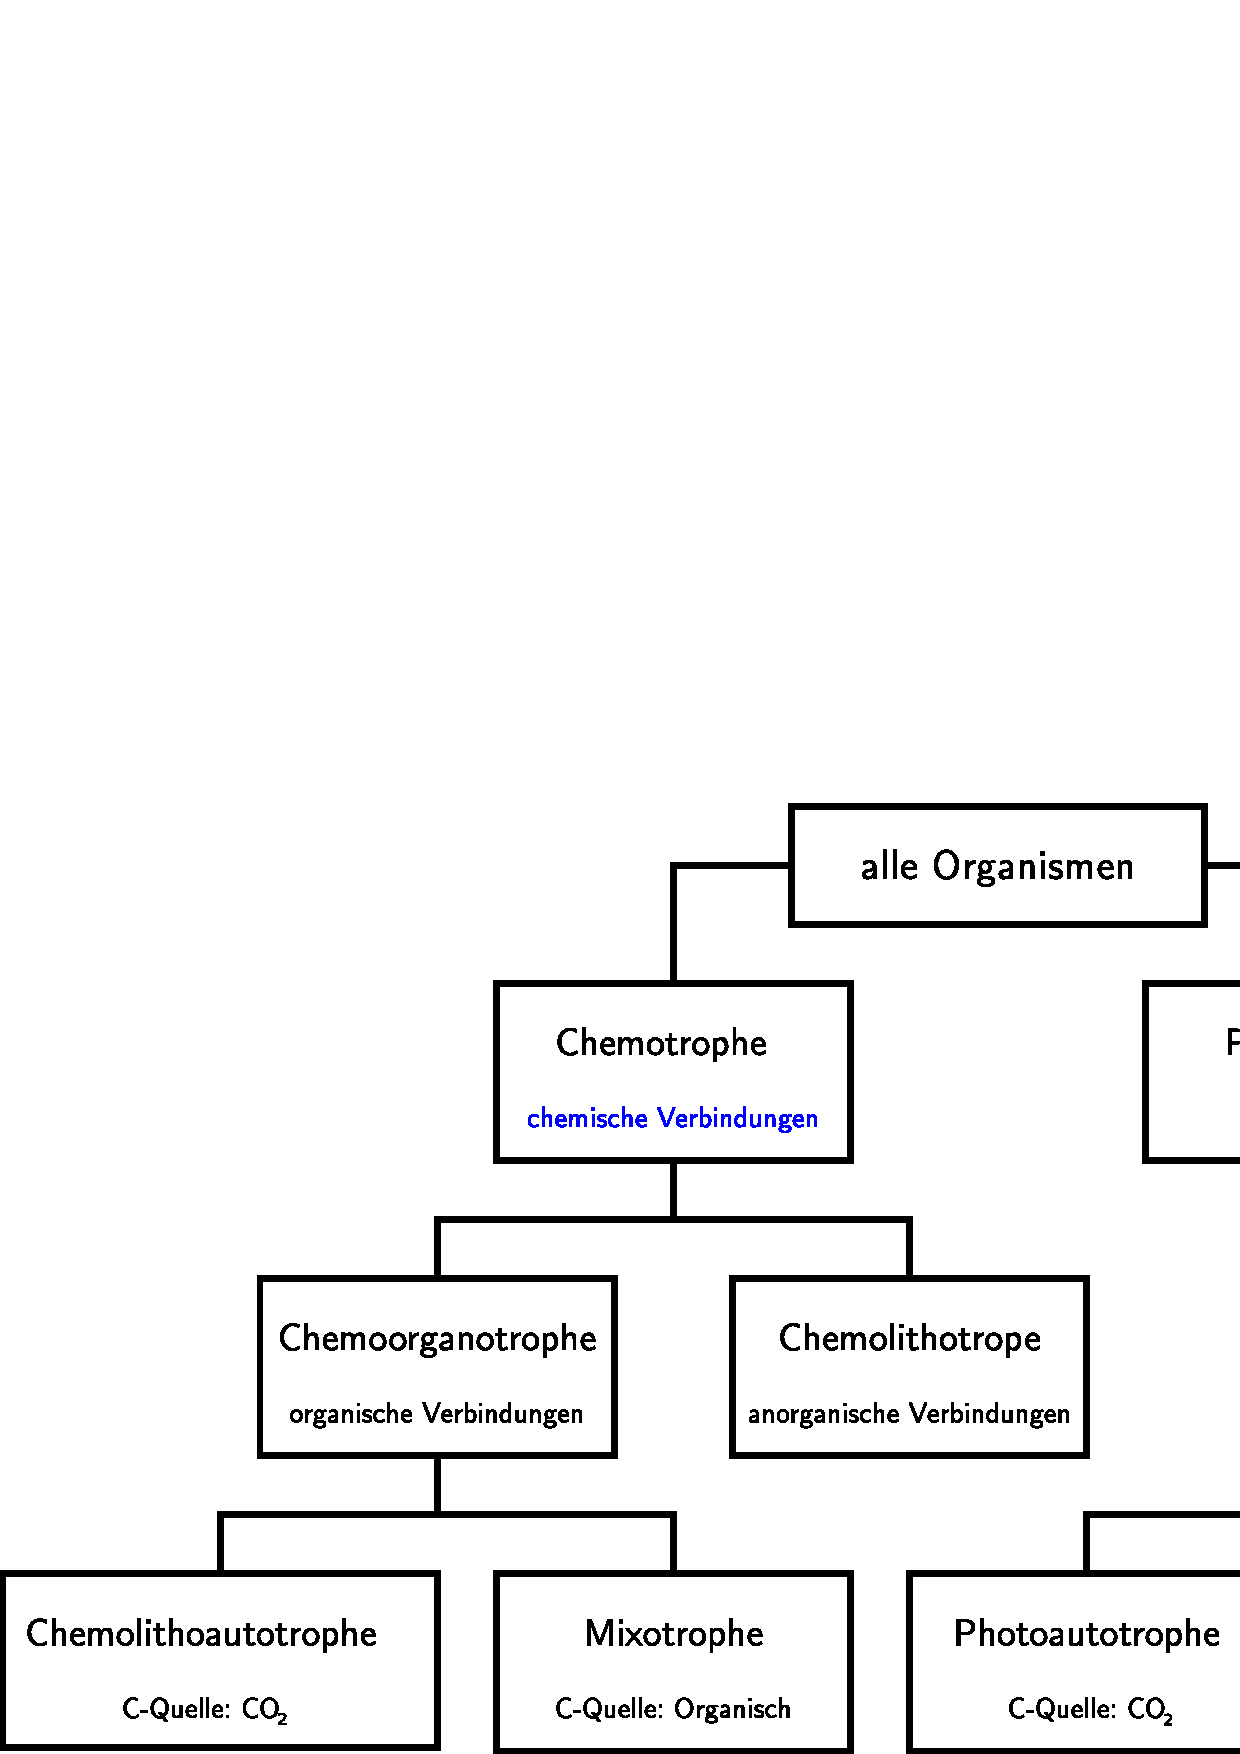
\includegraphics[scale=0.45]{./pictures/stoffwechsel.pdf}
		\end{center}
		\caption{\slshape{Stoffwechselvarianten von Mikroorganismen.
								Dargestellt sind die \textcolor{blue}{Energiequelle} und die Kohlenstoffquelle.}}
		\label{fig:Stoffwechselvarianten}
		\end{figure}

	\item[Substratkettenphosphorylierung]	\hfill	\\
		Bildung von ATP durch den direkten Transfer eines ernergiereichen
		Phosphatmoldeküls von einer phosphorylierten organischen Verbindung
		auf ADP.
		Typisch für Fermentation.
\end{description}


\end{document}
\end{input}
